\documentclass[12pt, a4paper, oneside]{ctexart}
\usepackage{amsmath, amsthm, amssymb, bm, color, enumerate, framed, graphicx, longtable, mathrsfs, subfigure, tikz}
\usepackage{geometry}
\geometry{left=2.54cm,right=2.54cm,top=3.18cm,bottom=3.18cm}

% 超链接设置
\usepackage{hyperref}
\hypersetup{  
    colorlinks = true,    % 更改链接颜色  
    linkcolor = purple,      % 链接颜色  
    urlcolor = blue,        % URL 颜色  
    citecolor = green,     % 引用颜色  
    % underline = true,  
    linkbordercolor = red,
}
% \hypersetup{colorlinks=true,linkcolor=black}

%代码包设置
\usepackage{listings}
\lstset{
    basicstyle          =   \sffamily,          % 基本代码风格
    keywordstyle        =   \bfseries,          % 关键字风格
    commentstyle        =   \rmfamily\itshape,  % 注释的风格,斜体
    stringstyle         =   \ttfamily,  % 字符串风格
    flexiblecolumns,                % 别问为什么,加上这个
    numbers             =   left,   % 行号的位置在左边
    showspaces          =   false,  % 是否显示空格,显示了有点乱,所以不现实了
    numberstyle         =   \zihao{-5}\ttfamily,    % 行号的样式,小五号,tt等宽字体
    showstringspaces    =   false,
    captionpos          =   t,      % 这段代码的名字所呈现的位置,t指的是top上面
    frame               =   lrtb,   % 显示边框
}
\lstdefinestyle{C}{
    language        =   C, % 语言选C
    basicstyle      =   \zihao{-5}\ttfamily,
    numberstyle     =   \zihao{-5}\ttfamily,
    keywordstyle    =   \color{blue},
    keywordstyle    =   [2] \color{teal},
    stringstyle     =   \color{magenta},
    commentstyle    =   \color{red}\ttfamily,
    breaklines      =   true,   % 自动换行,建议不要写太长的行
    columns         =   fixed,  % 如果不加这一句,字间距就不固定,很丑,必须加
    basewidth       =   0.5em,
}

% 设置思源宋体为中文字体
\setCJKsansfont{Source Han Serif SC}

% 设置思源黑体为中文字体
\setCJKsansfont{Source Han Sans SC}

% 设置arev为英文字体
\setsansfont{Arev Sans}

% 字体颜色
\def\red{\color{red}}
\def\blue{\color{blue}}
\def\black{\color{black}}
\def\green{\color{green}}

\title{\textbf{操作系统课程作业}}
\author{162140222黄钰轩}
\date{\today}
\linespread{1.25}

\definecolor{shadecolor}{RGB}{241, 241, 255}
\newcounter{problemname}
\newenvironment{problem}{\begin{shaded}\stepcounter{problemname}\par\noindent\textbf{题目\arabic{problemname}. }}{\end{shaded}\par}
\newenvironment{solution}{\par\noindent\textbf{解答. }}{\par}
\newenvironment{note}{\par\noindent\textbf{题目\arabic{problemname}的注记. }}{\par}
%\renewcommand{\proofname}{\bf 证明}

\begin{document}

\begin{figure}[t]
    \centering
    
\includegraphics[width=13cm]{images/logo.png}
\end{figure}

\maketitle

% \begin{problem}
%     如果有两个生产者,两个消费者,请改写下面的程序,消除竞争条件.
%     \lstinputlisting[
%         style       =   C,
%         caption     =   {\bf race.c},
%         % label       =   {probe.c}
%     ]{./code/data_race.c}
% \end{problem}

% \begin{solution}
%     \lstinputlisting[
%         style       =   C,
%         caption     =   {\bf race-solution.c},
%         % label       =   {probe.c}
%     ]{./code/data_race_solution.c}
% \end{solution}

\begin{problem}
    桌上有一空盘,只允许存放一个水果. 爸爸专向盘中放橙子,妈妈专向盘中放苹果,女儿专等吃橙子,儿子专等吃苹果. 规定当盘空时一次只能放一个水果供吃者自用,请用 P、V 操作实现爸爸、妈妈、女儿、儿子四个并发进程的同步.
\end{problem}

\begin{solution}
    具体代码如下:
    \lstinputlisting[
        style       =   C,
        caption     =   {\bf fruit.c},
        % label       =   {probe.c}
    ]{./code/fruit.c}
    \newpage
    执行结果下:
    \begin{figure}[!htbp]
        \centering
        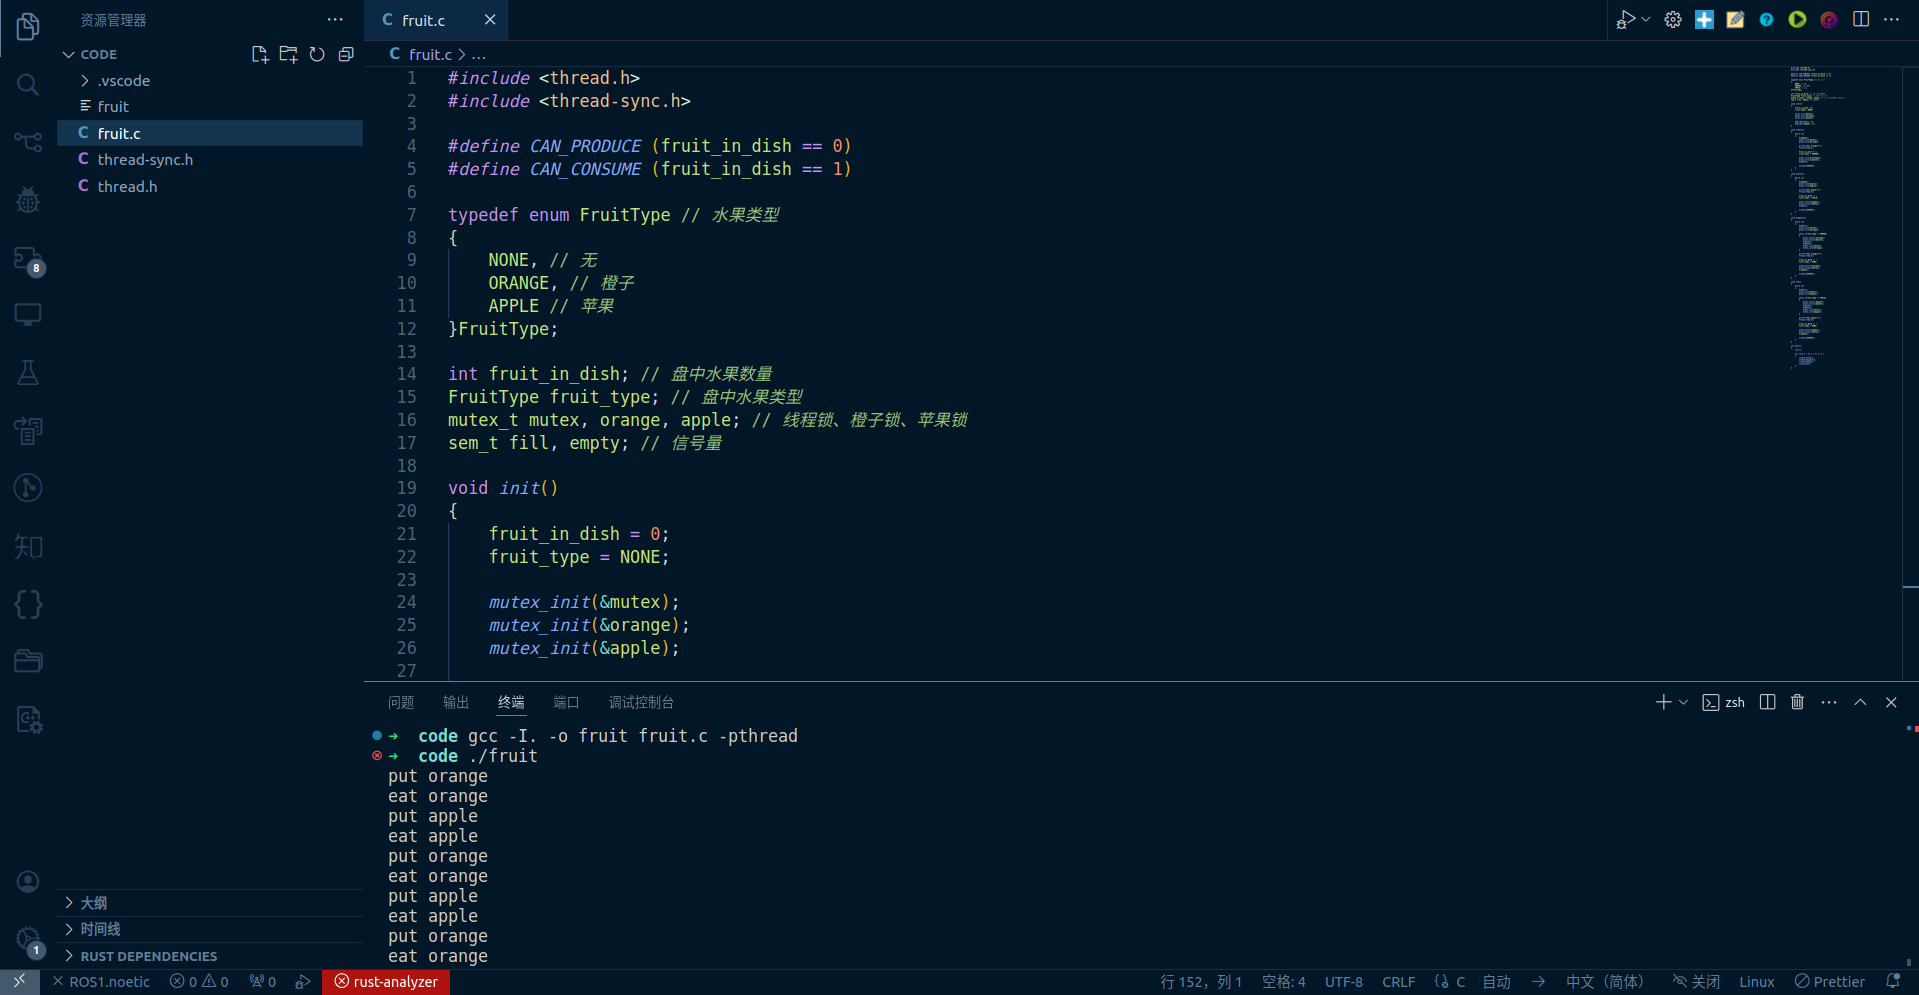
\includegraphics[width=15cm]{images/fruit.png}
        \caption{使用信号量实现同步}
    \end{figure}
\end{solution}

\begin{note}
    代码中所包含的头文件是一个将 POSIX 封装过后的\href{https://jyywiki.cn/os-demos/concurrency/thread-lib/}{“最简”线程库}. 本题的实现也参考了\href{https://jyywiki.cn/OS/2024/lect10.md}{2024南京大学操作系统}课程中的示例代码.
\end{note}

\begin{problem}
    假设有个南北向的桥,仅能容同方向的人顺序走过,相对方向的两个人则无法通过. 现在桥南北端都有过桥人,把每个过桥人当成一个进程,用 P、V 操作实现管理.
\end{problem}

\begin{solution}
    假定桥上最多允许3人同时通行,这里给出过桥过程的代码实现: 
    \lstinputlisting[
        style       =   C,
        caption     =   {\bf bridge.c},
        % label       =   {probe.c}
    ]{./code/bridge.c}
    \newpage
    执行结果下:
    \begin{figure}[!htbp]
        \centering
        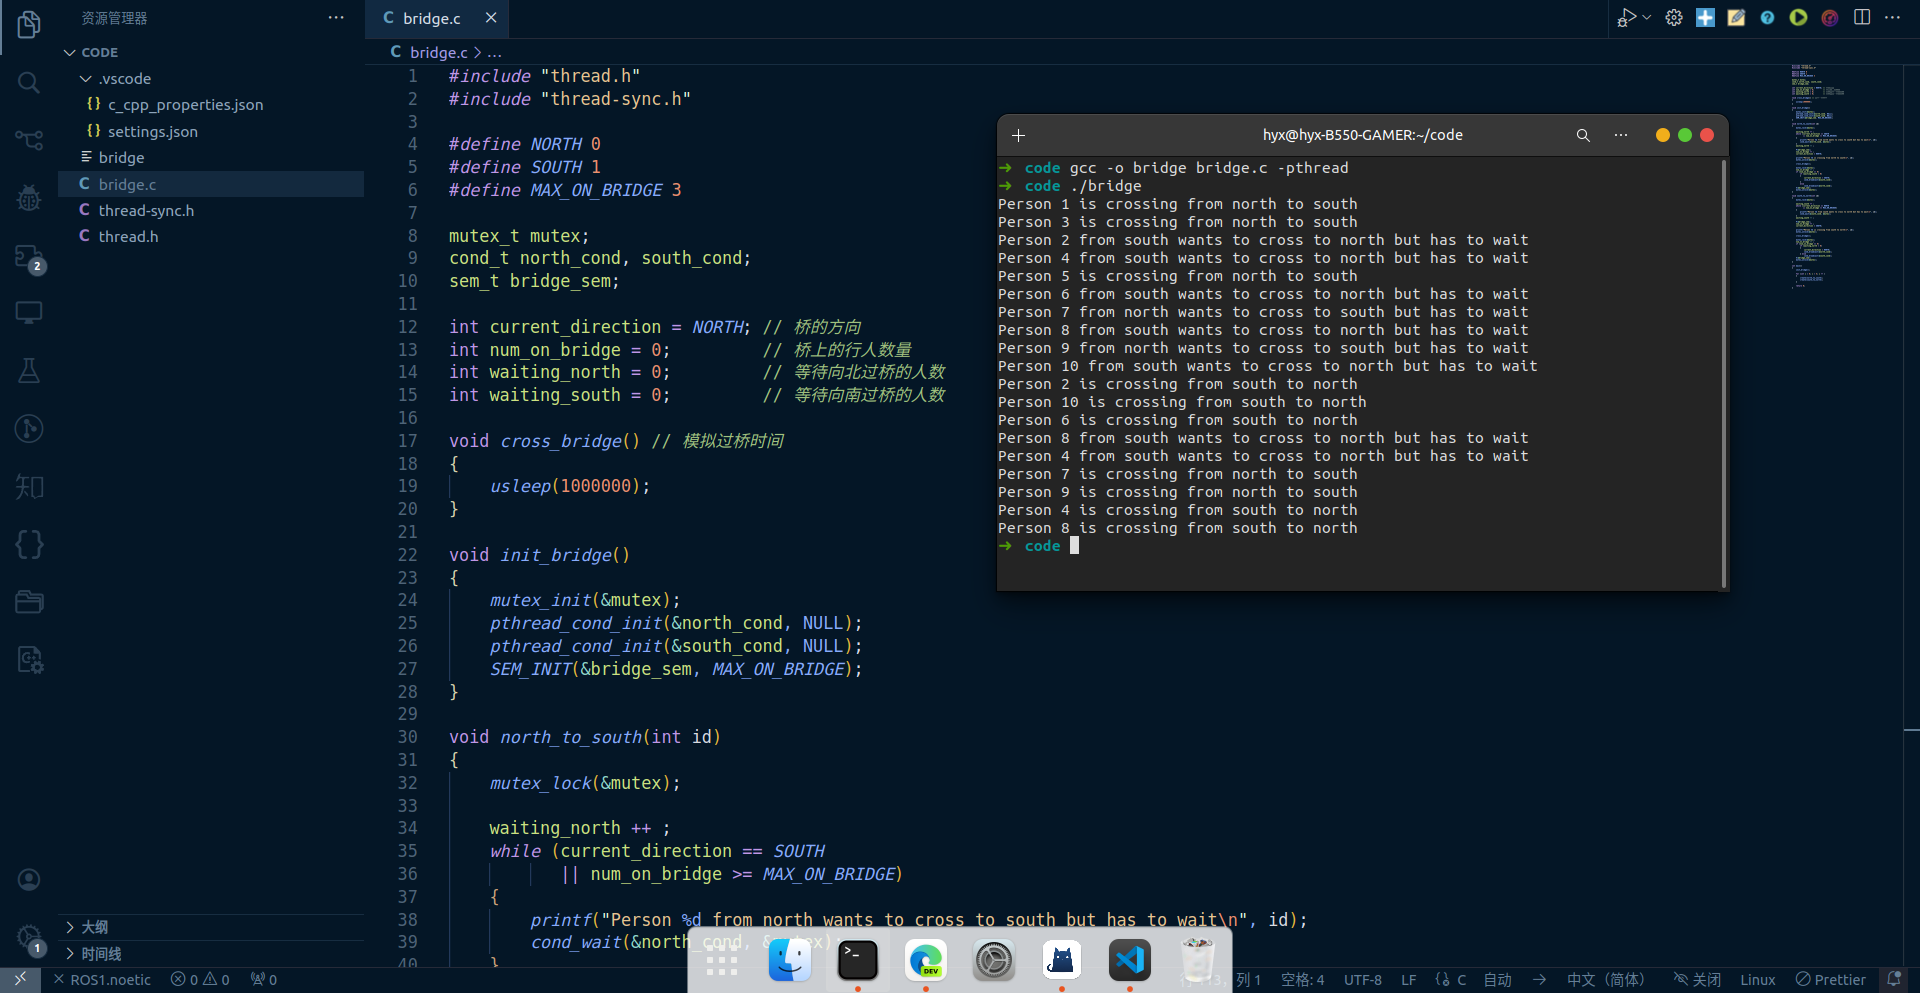
\includegraphics[width=15cm]{images/bridge.png}
        \caption{过桥问题}
    \end{figure}
\end{solution}

\end{document}